\documentclass[a4paper,11pt]{article}

%---Packages utilisés
\usepackage[utf8]{inputenc}
\usepackage[T1]{fontenc}
\usepackage[frenchb]{babel}
\usepackage{indentfirst}
\usepackage[]{graphicx}
\usepackage{amsmath}
\usepackage{ccaption}
\usepackage{vmargin}
\usepackage{textcomp}
\usepackage{fancyhdr}
%\usepackage[avantgarde]{quotchap}
\usepackage[Lenny]{fncychap}
\usepackage{cite}
\usepackage{siunitx}
\usepackage{hyperref}

\fancypagestyle{plain}{
\fancyhead[]{}
\fancyfoot[R]{\thepage}
\renewcommand{\headrulewidth}{0pt}}

%---Nouvelles commandes
\newcommand{\arronax}{\textsc{Arronax}}
\newcommand{\cyrce}{\textsc{Cyrcé}}
\newcommand{\Root}{\textsc{Root}}
\renewcommand{\baselinestretch}{1.2}

%\renewcommand{\chaptermark}[1]{%
% \markboth{\thechapter . \ #1}{}}

%---Mise en page
\setlength{\parindent}{2ex}
%\pagestyle{fancy}

%---Début du document
\begin{document}

%---Marges du document
\setmarginsrb{3.5cm}{1.5cm}{1.5cm}{2cm}{2ex}{3ex}{2ex}{5ex}
%1 est la marge gauche
%2 est la marge en haut
%3 est la marge droite 
%4 est la marge en bas
%5 fixe la hauteur de l'etête
%6 fixe la distance entre l'entte et le texte
%7 fixe la hauteur du pied de page
%8 fixe la distance entre le texte et le pied de page
%
%\chapterstyle{veelo}
%\renewcommand{\sectionmark}[1]{\markright{\thesection\ #1}}
\lhead[]{}
\fancyfoot[C]{}
\fancyfoot[R]{\thepage}

%%%%%%%%%%%%%%%%
\begin{center}
\subsection*{Pense-bête}
\end{center}

\subsubsection*{Electromètres}
La limite de fonctionnement d'un électromètre est de 12 pC par intégration. 
Une intégration peut durer au minimum 20 $\mu$s, mais les 32 électromètres fonctionnant par paire de 16, 40 $\mu$s sont nécessaires pour obtenir une mesure complète des 32 voies.
Augmenter ce temps d'intégration permet de diminuer le bruit sur les voies.
Multiplier le nombre d'intégrations lui ne fait que multiplier le bruit par le même facteur. 
\`A titre d'exemple, le bruit moyen pour une intégration est de 0.21 pC, avec 120 intégrations (fonctionnement de base) nous retombons bien sur une valeur de bruit d'environ 25 pC que nous observons sur les électromètres.

\subsection*{Intensité faisceau limite}
12 pC par 20 $\mu$s ou pour être exact 24 pC par 40 $\mu$s correspondent à différentes valeurs d'intensité de faisceau, suivant la nature de celui-ci, ainsi que les caractéristiques du Dosion (principalement son épaisseur).
Le type de particules primaires, leur énergie, ou même sa diffusion spatiale (faisant qu'il va frapper plus ou moins de pistes) sont à prendre en compte.

Dans le cas de protons, et en considérant la limite pour une seule piste, nous devons d'abord déterminer le nombre de paires électron-trou créées lors du passage d'une particule dans le gap de Dosion.
C'est notamment là qu'interviennent les caractéristiques du détecteur utilisé, à savoir l'épaisseur de son gap et la nature du gaz le constituant.
Pour le gaz, pour l'instant seul l'air est utilisé. 
Les gaps peuvent eux être de 3 mm ou 5 mm.

Connaissant la nature du gaz, nous pouvons nous référer au site du \href{https://physics.nist.gov/PhysRefData/Star/Text/PSTAR.html}{NIST} pour obtenir les tables de perte d'énergie des particules, comme pour les protons dans l'air représenté sur la figure \ref{fig:pAir} dont certaines valeurs sont listées dans le tableau \ref{tab:pAir}.

\begin{figure}
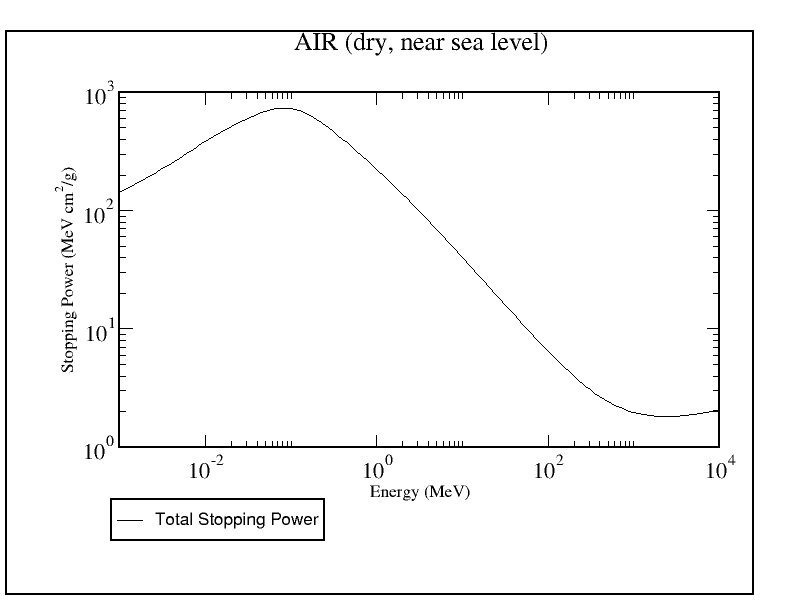
\includegraphics[width=\linewidth]{pAir.png} 
\caption{\label{fig:pAir}\footnotesize{Perte d'énergie des protons dans l'air.}}
\end{figure}

\begin{table}[h]
\begin{center}
\begin{tabular}{r@{.}lr@{.}ll|rr}
\multicolumn{2}{c}{MeV}&\multicolumn{2}{c}{MeV$\cdot$cm$^2\cdot$g$^{-1}$}&&3 mm&5 mm\\
\hline
\hline
4&5&\hspace*{3ex}74&88&limite basse Cyrcé&786&1310\\
10&0&40&0&&420&700\\
25&0&19&14&limite haute Cyrcé&201&335\\
70&0&8&44&limite haute Arronax&89&148\\
200&0&3&974&limite haute CPO&42&70\\
\hline
\end{tabular}
\caption{\label{tab:pAir}\footnotesize{Perte d'énergie et nombre moyen de paires électron-trou créées par des protons dans l'air pour certaines énergies usuelles et en fonction des tailles de gaps possibles.}}
\end{center}
\end{table}

Connaissant la densité de l'air, 1.225$\cdot$10$^{-3}$ g$\cdot$cm$^{-3}$, et le potentiel d'ionisation de l'air pour une particule chargée lourde, 35 eV, nous pouvons obtenir le nombre moyen, N$_{eh}$ de paires électron-trou créées :
$$N_{eh}=\frac{[MeV\cdot cm^2\cdot g^{-1}]\cdot 1.225\cdot 10^{-3} g\cdot cm^{-3}}{35\cdot 10^{-6}\ MeV}\cdot gap$$

Les valeurs obtenues sont répertoriées dans le tableau \ref{tab:pAir}.
Il ne faut pas oublier que Dosion fonctionne avec un double gap, donc que le nombre de paires doit être doublé pour chaque piste.

Chacune de ces paires va générer un signal de e=1.602$\cdot$10$^{-19}$ C sur la piste concernée.
Nous pouvons ainsi calculer l'intensité limite  suivant la formule :
$$I_l[proton\cdot piste^{-1}\cdot s^{-1}]=\frac{24\ pC}{e\cdot N_{eh}\cdot 40\ \mu s}$$

\begin{table}[h]
\begin{center}
\begin{tabular}{r@{.}lr@{.}lr@{.}l}
\multicolumn{2}{c}{MeV}&\multicolumn{2}{c}{3 mm}&\multicolumn{2}{c}{5 mm}\\
\hline
\hline
4&5&\hspace*{3ex}2&38$\cdot$10$^9$&\hspace*{3ex}1&43$\cdot$10$^9$\\
10&0&4&46$\cdot$10$^9$&2&68$\cdot$10$^9$\\
25&0&9&32$\cdot$10$^9$&5&59$\cdot$10$^9$\\
70&0&2&11$\cdot$10$^{10}$&1&27$\cdot$10$^{10}$\\
200&0&4&49$\cdot$10$^{10}$&2&69$\cdot$10$^{10}$\\
\hline
\end{tabular}
\caption{\label{tab:pAirI}\footnotesize{Intensité maximale supportée par les électromètres en nombre de protons par piste par seconde suivant l'énergie des protons incidents.}}
\end{center}
\end{table}

\end{document}